\documentclass{sig-alternate}

\usepackage{amsmath}
%\usepackage{amsthm}
\usepackage{listings}
\usepackage{tikz}
\usepackage{subfigure}
\usepackage{multirow}
\usepackage{pgfplots}
\usepackage{booktabs}
\usepackage{dcolumn}
\usepackage{cancel}
\usepackage{graphics}
\usepackage{url}

\newcommand{\infrule}[2]{\displaystyle\frac{\displaystyle\strut{#1}}{\displaystyle\strut {#2}}}
\newcommand{\deref}{\ast}
\newcommand{\rread}[1]{\mbox{\em Read}(#1)}
\newcommand{\rwrite}[1]{\mbox{\em Write}(#1)}
\newcommand{\lca}[2]{#1 \sqcup #2}
\newcommand{\rleq}{\leq}
\newcommand{\interval}[1]{\mbox{\em interval}(#1)}
\newcommand{\context}[1]{\mbox{\em context}(#1)}
\newtheorem{theorem}{Theorem} 
\newtheorem{lemma}[theorem]{Lemma}

\setlength{\pdfpagewidth}{8.5in}
\setlength{\pdfpageheight}{11in}

\pagenumbering{arabic}

\begin{document}

\title{High-Performance Language Primitives for Distributed Architectures using Asynchronous Events}
% Commented out for double-blind goodness
%% \numberofauthors{3}
%% \author{
%% \alignauthor Sean Treichler\\
%%              \affaddr{Stanford University} \\
%%              \email{sjt@cs.stanford.edu}
%% \alignauthor Michael Bauer \\
%%              \affaddr{Stanford University} \\
%%              \email{mebauer@cs.stanford.edu}
%% \alignauthor Alex Aiken \\
%%              \affaddr{Stanford University} \\
%%              \email{aiken@cs.stanford.edu}
%% }
\maketitle

\begin{abstract}
%The limit is 12 pages, including bibliography and appendices.
%Deadlines:
%\begin{tabular}{ll}
%Abstract deadline & July 16, 2012 3pm PDT \\
%Paper deadline & July 23, 2012 3pm PDT \\
%Author response & around October 15, 2012 \\
%Author notification & November 9, 2012
%\end{tabular}
We present a low-level runtime interface for current highly distributed, heterogeneous
parallel machines that provides a fully asynchronous 
programming model, allowing all types of runtime actions, including synchronization,
to be non-blocking.  Our interface includes mechanisms for the creation and movement
of data through the memory hierarchy as well as {\em deferred locks}, a novel synchronization primitive.
Asynchrony is exposed by the interface using a distributed event system.  All
operations return an event to be triggered when the operation completes.  Events
can be chained together and used to capture dependences between operations.

We describe an implementation of our interface capable of running on
a large supercomputer with both CPU and GPU processors and a high speed interconnect.
We employ several micro-benchmarks to show that our implementation approaches
the performance limits of the underlying hardware.
We also demonstrate that the interface is sufficiently powerful to serve as the foundation 
of an advanced parallel programming system.  We measure the performance of three real-world applications
that use our system on the Keeneland supercomputer.
\end{abstract}

%\section{Outline}

\begin{enumerate}
\item Abstract
\item Introduction
\item LLR Components
  \begin{enumerate}
  \item Processors
  \item Memories
  \item Events
  \item Locks
  \item Physical Regions
  \end{enumerate}
\item Implementations
  \begin{enumerate}
  \item SMP Version
  \item GASNet/CUDA Version
  \end{enumerate}
\item Microbenchmarks
  \begin{enumerate}
  \item Events
    \begin{enumerate}
    \item Latency (inter- and intra-node)
    \item Throughput (separate tracks and single wide track)
    \end{enumerate}
  \item Locks
    \begin{enumerate}
    \item Latency, Throughput vs. Load
    \item Locality - associate data with lock either implicitly or explicitly, show effect of unfairness
    \end{enumerate}
  \item Reductions
    \begin{enumerate}
    \item Histogram Mini-app - vary data, histogram sizes, use variety of reduction techniques
    \end{enumerate}
  \end{enumerate}
\item Applications
  \begin{enumerate}
  \item Circuit
  \item Fluid
  \item AMR
  \end{enumerate}
\item Application Profiling
  \begin{enumerate}
  \item Events
    \begin{enumerate}
    \item Lifetimes (Storage Cost)
    \item Trigger vs. Query Times
    \item Waiters per Event (individual and aggeregated per-node)
    \end{enumerate}
  \item Locks
    \begin{enumerate}
    \item ???
    \end{enumerate}
  \item Reductions
    \begin{enumerate}
    \item ???
    \end{enumerate}
  \item Deferred Execution
    \begin{enumerate}
    \item Comparison vs. Bulk Synchronous Implementation
    \end{enumerate}
  \end{enumerate}
\item Related Work
\item Conclusion
\item Bibliography
\end{enumerate}

\section{TODO}

\newcommand{\tblhdr}[1]{\multicolumn{1}{c}{\bf #1}}

\begin{tabular}{lll}
\tblhdr{Status} & \tblhdr{Owner} & \tblhdr{Task} \\
DONE & Mike & Code event latency microbenchmark \\
& Mike & Code event throughput microbenchmark \\
& ?? & Code lock latency/throughput microbenchmark \\
& Sean & Code lock locality microbenchmark \\
& ?? & Code histogram microbenchmark \\
& Sean & Detailed event logging \\
& Sean & Bulk-Synchronous Mode: Circuit \\
& Sean & Bulk-Synchronous Mode: Fluid \\
& Mike & Bulk-Synchronous Mode: AMR \\
\end{tabular}


\section{Introduction}
\label{sec:intro}

% Big machines -> latencies are growing
% Processors can't be blocked, need to be able to continue handling work
% Operations need to be composable
% deferred execution model

% Contributions:
% - An event system where every operation can take an event and returns an event
% - Handles are globally valid
% - More flexible synchronization primitive for this environment: deferred locks
% - Physical regions for data movement including special versions for reductions

% Parallel programs have three parts
%  Parallel control
%  Data movement in the memory hierarchy
%  Synchronization

% Bulk-synchronous
% asynchronous components are not composable

A characteristic feature of current and future heterogeneous
supercomputers is the large, variable, and growing latencies between
components.  The well-known mechanism for masking unpredictable or
long latencies is to use {\em asynchronous operations} that do not block,
thereby enabling other useful work to be done while the asynchronous
operations complete. Current implementation primitives for parallel
programming systems, however, rely on blocking constructs that were
designed for machines many orders of magnitude
smaller\cite{MPI,COARRAY_FORTRAN,UPC99}; these primitives expose
latency on today's large, distributed parallel machines.


Most current programming systems for large-scale parallel processing provide some variant
of the {\em bulk-synchronous} execution model\cite{Valiant90}.  Bulk-synchronous models
partition computations into {\em phases} that are either parallel computation, data
communication, or synchronization.  At any given point in time all processors
are engaged in the same kind of phase.  Bulk-synchrony
makes it easy to reason about parallel execution but
hinders attempts to hide the increasingly long-latency communication
or memory movement phases.  
%In older machines this was not a problem because slower
%processors and smaller machines meant computation phases were much larger than
%communication or synchronization phases.  However, today's machines are much
%larger with faster processors, causing an increasing percentage of time
%to be spent in the communication and synchronization phases.

To combat this problem, parallel programming libraries have introduced
asynchronous constructs allowing programmers to overlap phases.  For
example, MPI has asynchronous {\em send} and {\em receive} operations
for sending messages in parallel with computation \cite{MPI}.  There
are two problems with this approach.  First, not all phases support
asynchronous constructs.  Second, the asynchronous operations do not
compose.  There is no way to express that one asynchronous computation
should begin as soon as another asynchronous communication operation
has completed.  The result is that at some point there must be
blocking operations to coordinate synchronous and asynchronous phases.
If blocking calls are not accurately placed in the program they can
lead to processor stalls that expose latency.  Placement of blocking
calls is difficult to reason about because 
they can be dependent on input data, algorithmic decisions, 
and the underlying hardware.  Instead, to hide as much
latency as possible and to minimize processor stalls, 
%regardless of inputs, algorithmic choices, or underlying hardware,
all three major aspects of parallel programs (computation, data movement,
synchronization) should be asynchronous and composable.

We propose a new low-level interface for programming modern
supercomputers that is fully asynchronous. In our system, one can
asynchronously compose computation, data movement, and
synchronization.  The basic mechanism that enables composition of 
asynchronous operations
is an {\em event} primitive.  Events provide a mechanism
for naming a point in the future when an asynchronous operation
(computation, data copy, or synchronization) will complete.  Every
call to perform an operation $p$ in our runtime returns immediately
with an event that {\em triggers} when $p$ has completed.
Furthermore, every call to perform an operation $p$ can take as a
precondition an event that must trigger before $p$ can begin.
Any number of operations can be depedendent on a single event, and
a events can be merged to allow an operation to wait for multiple
events before it begins.
  Using
events clients can compose arbitrary chains of dependent
operations, which the runtime is free to execute in any way that
respects the event dependences.  With this freedom the runtime can
schedule operations to optimize throughput while hiding the long
latency operations.

The following sections describe our contributions:
\begin{itemize} \itemsep1pt \parskip0pt \parsep0pt
\item We present an interface for asynchronously composing
parallel computation, data movement, and synchronization using events (Section~\ref{subsec:events}).  

\item To support synchronization in our event system we introduce {\em deferred locks}, 
a novel synchronization primitive that operates in an asynchronous environment (Section~\ref{subsec:locks}).

\item We describe a physical region system that provides structural information about
data layout.  The structural information provided by physical regions enables an extensible
interface for conjoining operations on data (e.g. reductions) with asynchronous data movement for 
further latency hiding (Section~\ref{subsec:phyreg}).

\item Our approach depends on the efficient handling of very large numbers of events.
We describe a distributed implementation of our interface that requires no global coordination
and has modest local storage costs.  We describe optimizations for the implementation of events, 
deferred locks, and reductions (Section~\ref{sec:impl}).

\item We report on micro-benchmarks that are designed to stress
our implementation.  The results indicate that our implementation approaches the performance of
the underlying hardware (Section~\ref{sec:micro}).

\item We demonstrate that our interface is powerful enough to support Legion \cite{Legion12}, a higher-level
programming system, and that real Legion applications programmed to our interface
are capable of achieving high-performance (Section~\ref{sec:apps}).  Furthermore, we demonstrate
that the same applications written in a bulk-synchronous model incur performance penalties between 22-135\%.
\end{itemize}

Section~\ref{sec:related} describes related work and Section~\ref{sec:conclusion}
concludes.



\section{Programming Interface}
\label{sec:interface}
The target set of clients for our interface are higher-level language
compilers and runtimes such as Legion\cite{Legion12} as well as 
advanced systems programmers.  This class of clients expect total control
over the underlying hardware and transparent performance from an
implementation.  To support these demands we have designed our interface
to be as low-level as possible.  In many cases we have chosen to trade-off
ease of programmability for performance.  We eschewed any features that would
automatically be performed without being directed by the client.
Our goal in the design of this interface is to provide a set of low-level,
high-performance primitives that are asynchronous and composable.

Our interface organizes functionality into objects.  We describe
these objects in five parts: {\em events} for composing operations 
(Section~\ref{subsec:events}), {\em processors} for parallel computation 
(\ref{subsec:procs}), {\em deferred locks} for synchronization
(\ref{subsec:locks}), {\em physical regions} for data layout and movement
(\ref{subsec:phyreg}), and a {\em machine} object for introspection of the underlying
hardware (\ref{subsec:machmodel}).  In all cases (except for the
machine object which is a static singleton), instances of the objects
are light-weight {\em handles} that provide a unique name for an underlying
implementation.
Every handle is valid everywhere in the system, allowing handles to be freely copied,
passed as arguments to other tasks, or stored in the heap
without having to reason about the distributed nature of the system.
%%   Multiple copies of handles are permitted and handles can be 
%% passed by value.  Furthermore, every handle is valid everywhere in the system.  
%% This property allows a client to pass handles by value between computations 
%% without having to reason about the distributed nature of the system.
%We describe how we support this property in more detail in 
%Section~\ref{sec:impl}.

\lstset{
  captionpos=b,
  language=C++,
  basicstyle=\scriptsize,
  numbers=left,
  numberstyle=\tiny,
  columns=fullflexible,
  stepnumber=1,
  escapechar=\#,
  keepspaces=true,
  belowskip=-10pt,
  literate={<}{{$\langle$}}1 {>}{{$\rangle$}}1,
  %morekeywords={region,coloring,partition,spawn,disjoint,aliased},
  %deletekeywords=float,
}

\subsection{Events}
\label{subsec:events}
Events are the primary mechanism for describing dependences between operations in our system.
Listing~\ref{lst:eventapi} shows the interface for events.  An instance of the {\tt Event} type 
names a unique event in the system.  {\tt NO\_EVENT} (line 5) is a special instance
of an event that by definition has always triggered.  The event interface
supports testing whether an event has triggered (line 7) and waiting on
an event to trigger (line 9).  While these methods can be useful, the encouraged
use of events is passing them as preconditions for other operations.  The client can use the
{\tt merge\_events} call (lines 11-12) to create an event that triggers only when every
event in a given set of events has triggered.  An example using events follows in
Section~\ref{subsec:procs}.
%corresponding to the conjunction of a set of events.

In most cases events are created as the result of other
operations and the implementation is responsible for triggering these events.  Clients
can also create a {\tt UserEvent} (line 15) that is triggered explicitly by the client.

The common synchronization pattern in which multiple consumers are dependent on
a set of producers is supported by a {\tt Barrier} object, which is similar
to a user event, but does not trigger until the expected number of {\tt arrive}
operations have occurred.  To better support
composability and asynchronous operation, our interface differs from barriers in other programming
models\cite{MPI} in three fundamental ways:
%The common synchronization pattern in which multiple consumers are dependent on a 
%(potentially different) set of producers is supported by a {\tt Barrier} object,
%which is similar to a {\tt UserEvent}, but does not trigger until the expected
%number of {\tt arrive} operations have occurred.  Barrier constructs exist in other
%programming models\cite{MPI}, but in addition to the decoupling of the waiters from
%the arrivers, our barrier interface has two further improvements to better support
%composability and asynchronous operation:
\begin{itemize} \itemsep1pt \parskip0pt \parsep0pt
\item The set of producers of arrival calls can be different from the set of consumers waiting on the barrier.
\item An arrival operation can be made dependent on another event, allowing a client to
express that an operation should be completed before the barrier can trigger.
\item The expected arrival count of a barrier can be dynamically modified, allowing
barrier creation before needing to know the exact number of arrivals.
\end{itemize}

Both user events and barriers are a sub-type of events and can therefore
be used transparently to express dependences wherever events are used.
%Although user events and barriers are created and triggered differently,
%operations that express dependences on Events can transparently use
%UserEvents or Barriers as well.

%%   Users can also create another
%% type of event called a {\tt Barrier} that will require multiple arrivals before
%% the event is triggered.  The user can manage the number of arrivals that must
%% be seen as well as how many arrivals occur at a time.  Once a barrier's arrival
%% count goes to zero, the barrier will trigger.  Note that barriers in our interface
%% provide a superset of the functionality of traditional barriers since they can
%% be used in a blocking manner (via the {\tt wait} call), but are primarily used
%% asynchronously.  Lastly, since user events and barriers are sub-types of 
%% an event they can be used wherever an event is required.

\begin{lstlisting}[float={t},label={lst:eventapi},caption={Event Interface.}]
class Event {
public:
  const unsigned id;
  const unsigned gen;
  static const Event NO_EVENT;
  // check if an event has triggered
  bool has_triggered() const;
  // wait on the event
  void wait() const;
  // Merge events together to create a new event
  static Event merge_events(Event ev1, Event ev2);
  static Event merge_events(const set<Event> &to_merge);
};

class UserEvent : public Event {
public:
  static UserEvent create_user_event();
  void trigger() const;
};

class Barrier : public Event {
public:
  static Barrier create_barrier(unsigned expected_arrivals);
  void alter_arrival_count(int delta) const;
  void arrive(unsigned count = 1,
                  Event wait_for = Event::NO_EVENT) const;
};
\end{lstlisting}

\subsection{Processors}
\label{subsec:procs}
Listing~\ref{lst:procapi} shows the interface for {\tt Processor} objects which allow for
the creation of parallel computations.  Processors provide a way of naming 
every computational unit in the machine.  We describe how to discover processor handles
in Section~\ref{subsec:machmodel}.  In the case of our current interface 
processors are either individual cores or discrete GPUs, but this is easily modified 
to include new processor types (line 10).   Processors support a single {\tt spawn}
operation (lines 14-15) that launches a new {\em task} on that processor.
Note that because the spawn operation
is invoked on a processor handle, it is possible to launch a task on any
processor from anywhere in the system.  
The spawn call takes an optional event that must trigger before the task can begin.  
The spawn call returns an event that will trigger when the task completes.

Lines 18-24 of Listing~\ref{lst:procapi} show a simple example using 
the processor and event interface.  The {\tt diamond\_task} launches four
sub-tasks with a diamond dependence pattern, as shown in Figure~\ref{fig:procevents}.
The {\tt merge\_events} call
merges the events {\tt eb} and {\tt ec} to create the shared dependence
for the last sub-task.

\begin{lstlisting}[float={t},label={lst:procapi},caption={Processor Interface and Example.},belowskip=0pt]
class Processor {
public:
  const unsigned id;
  typedef unsigned TaskFuncID;
  typedef void (*TaskFuncPtr)
            (const void *args,size_t arglen,Processor p);
  typedef map<TaskFuncID, TaskFuncPtr> TaskIDTable;

  enum Kind {
    CPU_PROC,GPU_PROC,// ... future processor types
  };
  Kind kind() const;

  Event spawn(TaskFuncID func_id,const void *args,size_t arglen,
              Event wait_on = Event::NO_EVENT) const;
};

void diamond_task(const void *args,size_t arglen,Processor p){
  Event ea = p.spawn(TASK_A,NULL,0);
  Event eb = p.spawn(TASK_B,NULL,0,ea);
  Event ec = p.spawn(TASK_C,NULL,0,ea);
  Event em = Event::merge_events(eb,ec);
  Event ed = p.spawn(TASK_D,NULL,0,em);
}
\end{lstlisting}

\begin{figure}
\centering
\scalebox{0.8}{
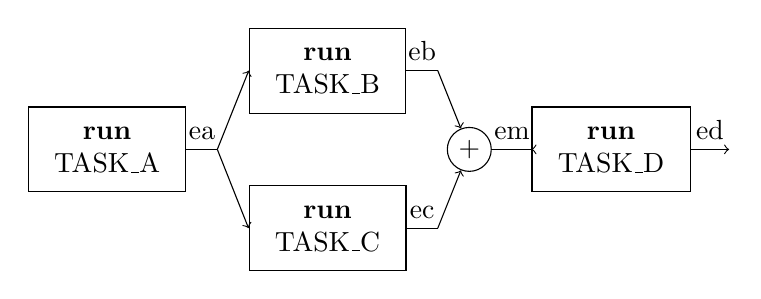
\begin{tikzpicture}
  %\path (1,3) node (t1) [shape=rectangle,draw] {run TASK\_A} -- node [right=1pt] {ea} +(0,-0.5) node[auto] {eax};
  \node (t1) at (0,0) [shape=rectangle,draw] {\begin{tabular}{c}{\bf run}\\TASK\_A\end{tabular}};
  \draw (t1) to node[auto] {ea} (1.4,0);

  \node (t2) at (2.8,1) [shape=rectangle,draw] {\begin{tabular}{c}{\bf run}\\TASK\_B\end{tabular}};
  \draw (t2) to node[auto] {eb} (4.2,1);
  \draw [->] (1.4,0) to (t2.west);

  \node (t3) at (2.8,-1) [shape=rectangle,draw] {\begin{tabular}{c}{\bf run}\\TASK\_C\end{tabular}};
  \draw (t3) to node[auto] {ec} (4.2,-1);
  \draw [->] (1.4,0) to (t3.west);

  \node (t4j) at (4.6,0) [shape=circle,inner sep=2pt,draw] {+};
  \draw (t4j) to node[auto] {em} (5.4,0);
  \draw [->] (4.2,1) to (t4j);
  \draw [->] (4.2,-1) to (t4j);

  \node (t4) at (6.4,0) [shape=rectangle,draw] {\begin{tabular}{c}{\bf run}\\TASK\_D\end{tabular}};
  \draw [->] (t4) to node[auto] {ed} (7.9,0);
  \draw [->] (5.4,0) to (t4.west);
  %
\end{tikzpicture}
}
\vspace{-2mm}
\caption{Processor Example Event Graph\label{fig:procevents}}
\vspace{-4mm}
\end{figure}

\subsection{Deferred Locks}
\label{subsec:locks}

Events and barriers express ordering properties between operations, but 
%in many cases 
ordering is often too strict a requirement.  For many applications access to data need only be atomic and
not necessarily ordered.  Traditionally locks have been used to serialize access to
data.  However, all lock implementations that we are aware of require either blocking
or spinning, neither of which composes well with asynchronous operations.
{\em Deferred locks} are a new synchronization mechanism that allows for synchronization
in an completely asynchronous environment.  

\begin{lstlisting}[float={t},label={lst:lockapi},caption={Deferred Lock Interface and Example.}]
class Lock {
public:
  const unsigned id;
  Event lock(Event wait_on = Event::NO_EVENT) const;
  void unlock(Event wait_on = Event::NO_EVENT) const;
  // Create a new lock, destroy an existing lock
  static Lock create_lock(size_t payload_size = 0);
  void *payload_ptr();
  void destroy_lock();
};

void launcher_task(const void *args, size_t arglen, Processor p) {
  ...
  // Unpack lock from arguments
  Lock needed = ...
  // Acquire lock
  Event lock_event = needed.lock();
  // Launch sub-task
  Event task_event = p.spawn(SUB,NULL,0,lock_event);
  // Release lock
  needed.unlock(task_event);
  ...
}
\end{lstlisting}

\begin{figure}
\centering
\scalebox{0.8}{
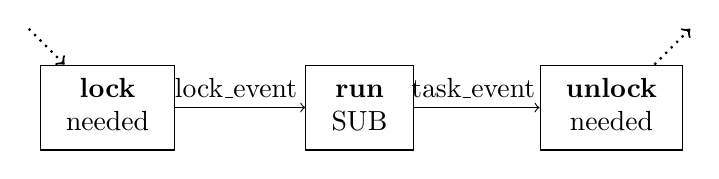
\begin{tikzpicture}
  %\path (1,3) node (t1) [shape=rectangle,draw] {run TASK\_A} -- node [right=1pt] {ea} +(0,-0.5) node[auto] {eax};
  \node (t1) at (0,0) [shape=rectangle,draw] {\begin{tabular}{c}{\bf lock}\\needed\end{tabular}};
  \draw (t1) to node[auto] {lock\_event} (2.4,0);

  \node (t2) at (3.2,0) [shape=rectangle,draw] {\begin{tabular}{c}{\bf run}\\SUB\end{tabular}};
  \draw (t2) to node[auto] {task\_event} (5.4,0);
  \draw [->] (2.4,0) to (t2.west);

  \node (t3) at (6.4,0) [shape=rectangle,draw] {\begin{tabular}{c}{\bf unlock}\\needed\end{tabular}};
  \draw [->] (5.4,0) to (t3.west);

  \draw [->,dotted,thick] (-1,1) to (t1.135);
  \draw [->,dotted,thick] (t3.45) to (7.4,1);
\end{tikzpicture}
}
\vspace{-2mm}
\caption{Lock Example Event Graph\label{fig:lockevents}}
\vspace{-4mm}
\end{figure}

Listing~\ref{lst:lockapi} shows the 
interface for locks.  Unlike blocking locks, the {\tt lock} method (line 4) doesn't
block but instead always returns immediately with an event that will be triggered
when the lock has been acquired.  Just like the spawn method, the lock method also 
takes an optional event parameter as a precondition.  Similarly, the {\tt unlock} 
method (line 5) takes an optional event precondition parameter.

An important difference between deferred locks and blocking locks is that the processor
that requests the lock doesn't have to be the one that uses it.  A common
convention in writing code with deferred locks is to acquire locks on behalf of a task being
launched.  Listing~\ref{lst:lockapi} illustrates this with a simple example.  The
{\tt launcher\_task} is calling a sub-task that is going to require the {\tt needed}
lock.  A lock request is issued and the resulting {\tt lock\_event} is used as
a precondition for launching the {\tt SUB} task.  The unlock operation is then
made dependent
%precondition
on the event corresponding to {\tt SUB} task's completion.  The
{\tt SUB} task can run safely while holding the lock and the lock is released when the
{\tt SUB} task completes.  Figure~\ref{fig:lockevents} shows the event dependence graph, with
dotted lines representing a lock operation's dependence on a previous unlock.
Using deferred locks in this style prevents 
compute resources from waiting on locks by ensuring tasks only run when their needed
locks have already been acquired.

When a lock is used to mediate access to a piece of data, the first thing a task will usually
do after being granted the lock is access the data.  To be able to hide the latency of that
access as well, an additional feature of locks in our interface is the association of a lock with a
{\em payload}, a small (i.e. less than 4KB) 
piece of data that is moved around with the lock and guaranteed to be coherent while 
the lock is held.  The size of the payload is specified when the lock is created (line 7) and
the pointer to the local copy of the payload can be obtained from the {\tt payload\_ptr} method
(line 8).

Between deferred locks and barriers (described in Section~\ref{subsec:events}) clients 
have access to the same set of synchronization primitives that they have
in threading and bulk-synchronous interfaces.  However, these operations can now 
be composed with other asynchronous operations which is not possible in any other interface
of which we are aware.

%Deferred locks provide a super-set of the functionality of blocking locks.  As their
%name suggests, deferred locks can use the event corresponding to their lock acquire
%operation to defer execution until the lock acquire has been granted.  Deferred
%locks can also be converted back into a blocking lock by immediately waiting on the event
%returned from a call to {\tt lock}.  In addition, deffered locks also provide {\tt mode} and
%and {\tt exclusive} parameters that allow the user to specify whether other requests can acquire
%the lock simultaneously.  A lock can only be acquired in one mode at a time.  The
%{\tt exclusive} parameter specifies whether other owners are permitted once the
%current lock request is granted.


\subsection{Physical Regions}
\label{subsec:phyreg}
In distributed machines with discrete memories, data movement often consists of more
than a simple copy operation.  Many applications perform operations and transformations on
their data in conjunction with data movement for higher performance.  One common example is 
that applications accumulate reduction operations in a buffer and then, as part of a copy operation,
the reduction operations are applied to a destination buffer on the receiving side of the copy.  
To support these kinds of conjoined operations in an asynchronous environment, our interface 
must be aware of the structure of data so it can perform accompanying operations with 
data movement operations.  To describe the structure of data our interface uses {\em physical regions.}

A physical region is an allocation of data in a single memory in the memory hierarchy.  Physical
regions are grouped into {\em classes} which are sets of physical regions that share the
same names (i.e. addresses) for elements, but don't necessarily share the same data layout.  This
allows pointers to elements within regions to be used, even if the regions are copied from one memory
to another.  Our
interface supports sub-classing, but the details are omitted due to space constraints.  The
interface allows copies between any pair of physical regions that are of
the same class (or between super- and sub-classes).  

%Note, clients can still pass arbitrary arrays
%of bits via the processor {\tt spawn} call.

% Say something about dynamically modifying the number of elements in a class

\begin{lstlisting}[float={t},label={lst:regionapi},caption={Physical Region Interface and Example.}]
class Memory {
public:
  const unsigned id;
  size_t size() const;
};

class RegionMetaData {
public:
  const unsigned id;
  static const RegionMetaData NO_REGION;
  // Create and destroy metadatas
  static RegionMetaData create_region(size_t num_elmts, 
                                      size_t elmt_size);
  void destroy_region() const;
  // Create and destroy instances
  RegionInstance create_instance(Memory memory) const;
  void destroy_instance(RegionInstance instance) const;
  // Create a physical instance only for reductions
  RegionInstance create_instance(Memory memory, 
                        ReductionOpID redopid) const;
};

class RegionInstance {
public:
  const unsigned id;
  static const RegionInstance NO_INST;
  // Copy between instances
  Event copy_to(RegionInstance target, 
                Event wait_on = Event::NO_EVENT);
};

template<typename LHS, typename RHS>
class ReductionOp {
public:
  static void apply(LHS *lhs, RHS rhs);
  // Optional methods for folding optimization
  static void fold(RHS *rhs1, RHS rhs2);
  static const RHS right_identity;
};

void reduction_ex(const void *args,size_t arglen,Processor p) {
  Memory m1,m2,m3; Processor p1,p2,p3; ReductionOpID redop = 2;
  ... // Choose memory and processors
  RegionMetaData meta = RegionMetaData::
                        create_region(num_elmts,elmt_size);
  Instance inst1 = meta.create_instance(m1,redop);
  Instance inst2 = meta.create_instance(m2,redop);
  Instance inst3 = meta.create_instance(m3);
  Event t1 = p1.spawn(REDUC,&inst1,sizeof(RegionInstance));
  Event t2 = p2.spawn(REDUC,&inst2,sizeof(RegionInstance));
  Event c1 = inst1.copy_to(inst3,t1);
  Event c2 = inst2.copy_to(inst3,t2);
  Event em = Event::merge_events(c1,c2);
  Event t3 = p3.spawn(USE,&inst3,sizeof(RegionInstance),em);
}
\end{lstlisting}

\begin{figure}
\centering
\scalebox{0.8}{
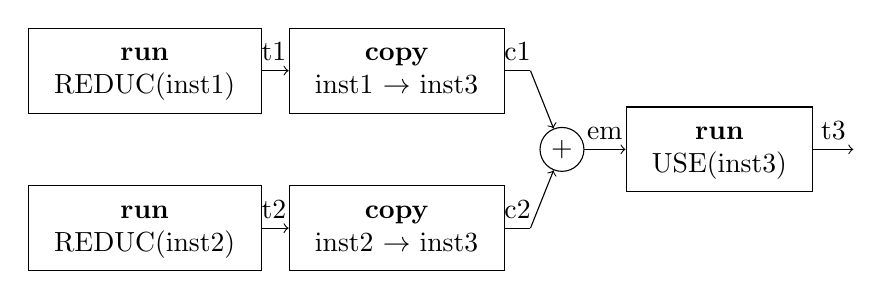
\begin{tikzpicture}
  %\path (1,3) node (t1) [shape=rectangle,draw] {run TASK\_A} -- node [right=1pt] {ea} +(0,-0.5) node[auto] {eax};
  \node (t1) at (0,1) [shape=rectangle,draw] {\begin{tabular}{c}{\bf run}\\REDUC(inst1)\end{tabular}};
  \draw (t1) to node[auto] {t1} (1.8,1);

  \node (t2) at (0,-1) [shape=rectangle,draw] {\begin{tabular}{c}{\bf run}\\REDUC(inst2)\end{tabular}};
  \draw (t2) to node[auto] {t2} (1.8,-1);

  \node (t3) at (3.2,1) [shape=rectangle,draw] {\begin{tabular}{c}{\bf copy}\\inst1 $\rightarrow$ inst3\end{tabular}};
  \draw (t3) to node[auto] {c1} (4.9,1);
  \draw [->] (1.8,1) to (t3.west);

  \node (t4) at (3.2,-1) [shape=rectangle,draw] {\begin{tabular}{c}{\bf copy}\\inst2 $\rightarrow$ inst3\end{tabular}};
  \draw (t4) to node[auto] {c2} (4.9,-1);
  \draw [->] (1.8,-1) to (t4.west);

  \node (t4j) at (5.3,0) [shape=circle,inner sep=2pt,draw] {+};
  \draw (t4j) to node[auto] {em} (6.1,0);
  \draw [->] (4.9,1) to (t4j);
  \draw [->] (4.9,-1) to (t4j);

  \node (t5) at (7.3,0) [shape=rectangle,draw] {\begin{tabular}{c}{\bf run}\\USE(inst3)\end{tabular}};
  \draw [->] (t5) to node[auto] {t3} (9,0);
  \draw [->] (6.1,0) to (t5.west);

\end{tikzpicture}
}
\vspace{-6mm}
\caption{Reduction Example Event Graph\label{fig:reducevents}}
\vspace{-4mm}
\end{figure}

Listing~\ref{lst:regionapi} shows a subset of the interface for physical regions.  
Each memory in the machine's memory hierarchy is named by a {\tt Memory} object (line 1).
The next object is a {\tt RegionMetaData} object (line 7), which defines a class of
regions.  Physical regions that belong to that class are created with the {\tt create\_instance}
method (line 16) and represented by {\tt RegionInstance} objects (line 23).  When creating a physical
region the client specifies the memory in which the physical region is going
to be allocated.  To maintain performance transparency, a new physical region can only be allocated
if the memory has sufficient capacity.
There is no automatic coherence of data between physical regions in the
same class.  It is the client's responsibility to manage data coherence using copies
between physical regions (line 28-29).  Like other operations copies can be
predicated on an event and return an event corresponding to completion.

If reductions are the only operations that will be performed on locations in a region instance,
a special reduction version can be created by providing the ID of a {\em reduction operator}
when the object is created (line 19).  Reduction-only region instances can 
increase the available parallelism and hide latency better, as we will show in 
section~\ref{subsec:reducmicro}.  The interface supports any reduction operation that
is commutative (i.e. multiple operations to the same location can be reordered without 
changing the final result) and is coded as an {\tt apply} method as shown on line 35.
Many commonly-used reduction operations are also {\em foldable} (e.g. $(l \text{ += } r_1) \text{ += } r_2$ can
be folded as $l \text{ += } r_1 + r_2$), and if the {\tt fold} operation and a {\em right identity}
(e.g. $0$ is a right identity for addition because $x + 0 = x$ for all $x$) are provided,
the runtime can use a {\em reduction fold instance}, described in section~\ref{subsec:reducimpl},
for even better performance.  Although the way they store data is very different,
reduction-only instances can be copied to other reduction-only instances (or normal 
instances) of the same class with the same asynchronous copy operations.  Copying between
instances with different layouts is only possible because physical regions provide 
the necessary information to understand the structure of the data.

%% Clients can also associate an operation as part of a physical region.  One example of
%% associating an operation with a physical region is shown on lines 13-14.  This instance
%% of the {\tt create\_instance} method
%% will create a physical region called a {\em reduction instance} that will be assoicated 
%% with the given {\tt ReductionOp} specified by the ID.  The interface for a {\tt ReductionOp} is shown on 
%% lines 26-33.  A reduction operation must have an {\tt apply} method, and can optionally 
%% implement two additional methods, {\tt init} and {\tt fold} that support additional 
%% optimizations described in Section~\ref{subsec:reducimpl}.  The two template parameters 
%% describe the base element type of the region ({\tt LHS}:left-hand-side) and the type of 
%% the argument to the reduction ({\tt RHS}:right-hand-side).  The reduction operation has 
%% total control over the choice of data layout for the reduction instance (not shown).
%% Reduction instances can be copied to other reduction instances with the same operation
%% or to regular physical regions of the same class.


An example using reduction-only regions is shown on lines 41-55 of Listing~\ref{lst:regionapi}.
Two reduction-only regions, {\tt inst1} and {\tt inst2}, are created in different memories to
be used with a reduction operation (lines 46-47).  A physical region of the same class {\tt inst3}
is also created in a different memory (line 48).  Two tasks are launched that will apply
reductions locally into their respective reduction buffers (lines 49-50).  The resulting
events are then used to chain copies back to {\tt inst3} after the tasks complete (lines 51-52).  As
part of these copies the reductions stored in {\tt inst1} and {\tt inst2} will be applied
to {\tt inst3}.  Since reductions are done atomically, there is no race between the reduction
applications.  Finally, a merge on the events from the movement and reduction applications is 
performed and a final task using {\tt inst3} is launched (lines 53-54).  The resulting event
graph is shown in Figure~\ref{fig:reducevents}.

%% SJT - redundant with first paragraph in this subsection?
%% Reductions and reduction instances illustrate only a single case where physical regions provide 
%% the structure necessary to conjoin an operation with data movement.  Physcal regions make our
%% interface easily extensible to arbitrary transformations and operations as a part of data movment.
%% While physical regions are a slightly higher-level construct than an annonymous
%% buffer of bits, we believe that the optimizations they enable are important in an asynchronous
%% environment.  Clients also still have access to an interface for controlling data layout through
%% the operations associated with physical regions which mitigates the loss in generality.

%{\em Physical regions} are the mechanism for reasoning about
%the placement and movement of data in the interface.  Physical regions are an 
%allocation of data in a single memory in the memory hierarchy.  Listing~\ref{lst:regionapi} 
%shows a subset of the physical region interface.  The first object in the interface
%is a {\tt RegionMetaData} object (line 1).  Region meta-data objects provide the interface for the
%creation of sets of physical regions that possess the same number and type of elements (but not necessarily
%the same data layout).  The interface is only able
%to copy data between two physical regions that were created by the
%same region meta-data object.  A runtime error will be generated if a copy is attempted
%between two physical regions that were not created by the same meta-data object.

%An instance of a physical region is represented by a {\tt RegionInstance} object (line 17).
%When creating a physical region the programmer must specify the {\tt Memory}
%in which the physical region is going to be allocated (line 10).  Memories are described
%in more detail in Section~\ref{subsec:machmodel}.  Once the physical region is created it
%cannot be moved.   There is no coherence of data between physical regions created by the 
%same meta-data object.  It is the programmer's responsiblity to manage data coherence
%using copies between physical regions (line 22-23).  Just like other operations,
%copies can be predicated on an event and return an event corresponding to
%completion.  
%A copy between two physical regions can only be performed if copies
%are permitted between the two memories where the regions were created.  
%The legality of copies can be discovered using queries to the {\tt Machine} object
%described in Section~\ref{subsec:machmodel}.

%The data held inside a physical region is accessed by another kind of object called an
%{\em accessor} (not shown).  Accessors support read, write, and reduction operations
%to elements inside the physical region.  Accessors can be specialized for the case where
%all memory is known to be directly accessible to the executing processor, which allows 
%for direct references to elements.  In cases where not all memory is directly accessable, 
%accessors supply the level of indirection necessary to convert operations into remote 
%memory operations (RMAs) if supported by the underlying hardware.  
%An example of this is described in more detail in Section~\ref{sec:impl}.

%One special (but common) case for applications is when reductions need to be performed.
%For reductions it is usually more efficient to store reduction
%operations in a local reduction buffer and then merge reduction buffers together at a later
%point in time.  To support this case the interface allows for the creation of a special kind
%of physical instance called a {\em reduction instance}.  The call to {\tt create\_instance} on
%lines 13-14 takes a {\em reduction operation} to be associated with a physical instance which
%tells the interface to create a reduction instance.  Reduction instances can only be accessed
%using a reduction of the given reduction type; any other accesses will result in a runtime
%error.  A reduction operation is a functor which must have at least one method of the type
%$(T_1 \rightarrow T_2 \rightarrow T_1)$ which takes a region element of type $T_1$ and a value
%to be reduced of type $T_2$ and creates and new region element.  Reduction operations can optionally 
%support two additional methods: a method that supplies an initial value of type $T_2$ and a 
%fold method of type $(T_2 \rightarrow T_2 \rightarrow T_2)$.  The presence of these methods
%enable additional optimizations for reductions described in Section~\ref{subsec:reducimpl}.

%Reduction instances can be copied using the same interface as regular physical instances.
%It is only legal to copy a reduction instance to a regular physical instance or another
%reduction instance of the same reduction operator.  Any attempt to copy from a regular physical 
%instance to a reduction instance will result in a runtime error.  A copy from a reduction 
%instance to a regular physical instance will apply all the reductions in the reduction 
%buffer to the physical instance.  If a copy is from one reduction instance to another, 
%the two reduction buffers will be merged.  The semantics of a merge are dependent upon 
%the underlying implementation of reduction buffers which is discussed in more detail 
%in Section~\ref{subsec:reducimpl}.




\subsection{Machine}
\label{subsec:machmodel}
The last component of the interface is shown in Listing~\ref{lst:machineapi} and allows the
initialization and run-time introspection
of the current machine.
The {\tt Machine} object is a singleton object that the client creates at the start of a
program, providing a task table that maps task IDs to function pointers,
and then invoking the {\tt run} method (lines 9-10).
Any running task can get a pointer to the machine object with the
{\tt get\_machine} method (line 12) and use it to obtain lists of all the {\tt Memory} (line 13) or 
{\tt Processor} (line 14) handles in the system.  Using the affinity methods (lines 16-19),
the application can also determine which memories are accessible by each
processor and with what performance, as well as which pairs of memories support copy operations.
%are able to efficiently copy data between themselves.

%% in the machine.
%% Second, the machine object provides an interface for the client to 
%% discover properties of the underlying machine (lines 35-43).  The machine object maintains
%% sets of all the unique {\tt Processor} and {\tt Memory} handles in the system.  Processors
%% were described in Section~\ref{subsec:procs}.  For every memory in the system there also 
%% exists a {\tt Memory} handle with a unique ID.  Different memories often, but not always, 
%% imply a different address space.  Examples of different memories are described in
%% Section~\ref{sec:impl}.

%For
%example, in a large cluster each node would have a different {\tt Memory} handle
%corresponding to each node's DRAM memory.
%However, if the cluster supported multiple GPUs then there would be a different
%{\tt Memory} handle for each GPU's {\em zero-copy} memory which shares part of the 
%address space with the corresponding node memory.  Memories will be used for describing
%the placement of data described in Section~\ref{subsec:phyreg}.

%The machine interface 
%contains three different object types: {\tt Processor} (line 1), {\tt Memory} (line 17), and a 
%singleton {\tt Machine} object (line 22).  For every processor (i.e. CPU core or GPU) in 
%the system there exists a {\tt Processor} handle with a unique ID naming that processor.  
%{\tt Processor} objects support a single {\tt spawn} operation (line 13-14) that will
%launch a {\em task} on that processor.   

%% The machine object also maintains two relations between the set of processors
%% and the set of memories:
%% \begin{itemize}
%% \item Processor-Memory: for each processor-memory pair whether
%% the processor can directly access (read and write) the memory and 
%% latency and bandwidth properties if access is possible
%% \item Memory-Memory: for every pair of memories whether copies can be
%% performed and latency and bandwidth properties if copies are possible
%% \end{itemize}
%%
%% The client can query these two relations by the {\tt get\_*\_affinity} calls
%% (lines 40-43) to discover properties of the machine.  

%These calls populate a vector with affinity structures (not shown)
%that contain latency and bandwidth information.  The programmer can restrict the query
%by specifying a specific processor or memory, otherwise information is returned
%about all processors and memories in the system.  

\begin{lstlisting}[float={t},label={lst:machineapi},caption={Machine Interface.}]
class Machine {
public:
  Machine(int *argc, char ***argv,
          const Processor::TaskIDTable &task_table);
  enum RunStyle {
    ONE_TASK_ONLY,ONE_TASK_PER_NODE,
    ONE_TASK_PER_PROCESSOR,
  };
  void run(Processor::TaskFuncID task_id = 0, 
        RunStyle = ONE_TASK_ONLY, const void *args, size_t arglen);
public:
  static Machine* get_machine(void);
  const set<Memory>& get_all_memories(void) const;
  const set<Processor>& get_all_processors(void) const;

  int get_proc_mem_affinity(vector<ProcMemAffinity> &result,
          Processor restrict_proc = 0, Memory restrict_mem = 0);
  int get_mem_mem_affinity(vector<MemMemAffinity> &result,
          Memory restrict_mem1 = 0, Memory restrict_mem2 = 0);
};
\end{lstlisting}




\section{Runtime Implementation}
\label{sec:impl}

There are currently two implementations of our interface:
one that works only on shared memory machines and another that
runs on larges clusters with both CPUs and GPUs.  The shared-memory
implementation uses the POSIX threads library.
The implementation for heterogeneous clusters also uses POSIX
threads as well as the CUDA runtime library for GPUs\cite{CUDA} and the GASNet
API for large clusters\cite{GASNET07}.  

The heterogeneous implementation
models a cluster with CPUs and GPUs as having two types of processors 
and four types of memory.  Every CPU core is a different CPU processor
and every GPU is a GPU processor.  For every node in the system
there is a memory corresponding to the DRAM associated with that node.  For
every GPU in the system there are two memories corresponding to the framebuffer
memory and the zero-copy memory associated with that GPU \footnote{Zero-copy 
memory contains pages that are mapped in both framebuffer and node memory with
coherence maintained by the PCI-E protocol.}. The last memory is 
a global GASNet memory that represents pages that have been registered 
with all nodes in the system for supporting remote memory accesses (RMAs).
The GASNet memory provides the illusion of global memory.  CPU processors
can directly access their node memory, all zero-copy memories for GPUs on
their node, and the GASNet memory.  GPU processors can only access their
framebuffer memory and their zero-copy memory.  Copies are permitted
between all pairs of memory except between any framebuffer memory and
the GASNet memory.

To support inter-node operations our implementation relies on GASNet active
messages for communication.  Active messages are a command and a payload
that are sent remotely and cause a handler to be run on the target node.
A simple example of our use of active messages can be illustrated by the 
{\tt spawn} call on a {\tt Processor} object.  Consider the case where {\tt spawn}
is invoked on a processor that is on a remote node.  This operation is converted into
an active message that contains all the information about the task launch.
When the active message is handled by the remote node, the task and all its
metadata are registered with the processor on which the task was launched.
While most of the implementation of our heterogeneous runtime is straight
forward, the next three sections describe in greater detail the nuances
of the implementation of events, locks, and reduction instances.

\subsection{Event Implementation}
\label{subsec:eventimpl}
Events are created on demand by each node.  The ID of the creating node is encoded
in the upper bits of each event's ID and the creating node is said to be the 
event's {\em owner}.  If an event is used as an argument to an
operation on a remote node then the remote node can determine the owner of 
the event and send an active message to become a {\em subscriber} of the event.  When a
remote node becomes a subscriber to an event it guarantees that it will receive an active
message from the event's owner when the event triggers.  To minimize the amount
of communication that occurs between nodes, each node remembers the events to which it
is subscribed and guarantees that it only subscribes to an event once.  In the case
where there may be many remote waiters on an event 
this can dramatically reduce the number of inter-node active messages.

When an event triggers, it automatically notifies all of the operations that are waiting
on its local node.  The owner node will also send active messages to all of the subscriber nodes
telling them that the event has triggered.  Even though the event has now notified all of
its waiters, the memory on the owning node for storing the event cannot be reclaimed 
because there still may be handles to the event in the system which will request to
use this event in the future.  These requests will need to be satisfied saying that 
the event has already triggered for the duration of the application.  Rather than waste
the resources, we recycle event implementations.

A {\em dynamic event} is a logical construct that will only be triggered once and is the level
of abstraction at which the programmer reasons about events.  A {\em physical event} is an
actual event implementation that consumes resources on its owner node.  Multiple dynamic events
can be mapped to a single physical event.  However, for each physical event there can be at most
one {\em active} event in the set of dynamic events that are mapped to it.  An active event is a 
dynamic event that is yet to trigger.  By only having one active dyanmic event at a time 
there is no need to disambiguate event triggers that are sent to the physical event.  Each
physical event maintains a count of the number of trigger operations that it has observed.

When the runtime needs to return a handle corresponding to a new dynamic event, it finds
a physical event which currently has no active events (e.g. the trigger count equals the number
of dynamic events mapped to the physical event).  The runtime increases the count
of the number of dynamic events mapped to the physical event.  The handle that is returned 
corresponds to a new dynamic event which contains an ID that refers to the physical
event it is mapped to and a {\em generation} that is the dynamic event number for the particular
physical event.  Note that by definition the generation will always be one greater than the
trigger count at the time of dynamic event creation.

Within this framework it is now very easy to test whether the dynamic event specified by a
handle has triggered.  Using the ID that is contained within the handle we find the
physical event implementation (which may require an active message if the owner node is
remote from where the test is begin performed).  We can then compare the generation of
the handle to the number of observed triggers contained by the physical event.  If the
number of physical triggers is greater than or equal to the handle's generation, then
the dynamic event has triggered.  We show in Section~\ref{sec:apps} that in practice
the number of needed physical events is significantly less than the number of dynamic events.

We also leverage the mapping of dynamic events onto physical events to improve the efficiency
of subscriptions.  Nodes cache the last generation for every physical event for which they
have seen a trigger notification.  If the trigger test described above detects a trigger based
on the cached information then there would be no need for the subscription which would save an
active message.  If the event has not been detected to have
triggered locally then an active message is sent to the owner which would always have been necesary
without the dynamic to physical event mapping.

\subsection{Lock Implementation}
\label{subsec:lockimpl}

\subsection{Reduction Instances}
\label{subsec:reducimpl}


\section{Benchmark Evaluation}
\label{sec:micro}

In this section we evaluate the heterogeneous implementation of our 
interface using several micro-benchmarks that test whether our implementation
approaches the underlying performance of the
hardware, and show that the optimizations described in Section~\ref{sec:impl}
are important.  All experiments were run on the Keeneland
supercomputer\cite{Keeneland}.  Each Keeneland node is composed of
two Xeon 5660 CPUs, three Tesla M2090 GPUs, and 24 GB of DRAM.  Nodes
are connected by an Infiniband QDR interconnect.

\subsection{Event Latency and Trigger Rates}
\label{subsec:eventmicro}
We implemented two micro-benchmarks for evaluating the performance of
events.  The first micro-benchmark tests the latency of event triggering,
both within a node and between nodes.  Processors are organized
into a ring and each processor in turn creates a user event that is dependent
on the previous processor's event.  The first event in this long chain of
dependent events is then triggered, and the time until the triggering of the
last event in the chain is measured.  The total time is divided by the number
of events in the chain to yield the mean trigger time.  In the single-node case, all events are local to
that node, so no active messages are required.  For all other cases, the
ring uses only a single processor per node so that every trigger requires
the transmission (and reception) of an event trigger active message.

%% is constructed.  The experiment measures the time from the triggering
%% of the first event to the triggering of the last event.  In the one node
%% configuration there is only one processor and all events are local to the
%% node.  In all other cases, there is only one processor per node which
%% guarantees that all event triggers result in an active message.  
%% Table~\ref{tab:eventlat} shows the results for both configurations.

\begin{figure}
\begin{center}
{ \small
\begin{tabular}{m{2cm}|c|c|c|c|c}
Nodes & 1 & 2 & 4 & 8 & 16 \\ \hline
Mean Trigger Time ($\mu$s) & 0.329 & 3.259 & 3.799 & 3.862 & 4.013 \\
\end{tabular}
}
\end{center}
\vspace{-6mm}
\caption{Event Latency Results.\label{tab:eventlat}}
\vspace{-4mm}
\end{figure}

\hyphenation{GASNet}

The calculated mean trigger times are shown in Table~\ref{tab:eventlat}.
The cost of manipulating the data structures themselves and running dependent
operations is shown by the single-node case, which experienced an average
latency of only 329 nanoseconds.  The addition of nearly 3 microseconds when
going from one node to two can be attributed to the latency of a GASNet
active message; others have measured similar latencies\cite{GASNET06}.
The gradual increase in latency with increasing node count is likely 
related to the underlying point-to-point nature of Infiniband communication,
which requires GASNet to poll a separate connection for every other node.
%% In the single node case the latency of triggering an event is only 
%% 329 nano-seconds.  For the multi-node cases, the triggering time is
%% between 3-4 micro-seconds which is the same as the cost of GASNet
%% active messages on Infiniband\cite{GASNET07}.  The gradual increase in latency with
%% node count is because each node must poll all the Infiniband connections for other nodes.
%% This cost of performing event triggers is in entirely in the hardware and the underlying software stack.

Our second micro-benchmark for events measures the maximum rate at which events can
be triggered by our implementation.  Instead of a single chain, many parallel chains
are created.  Additionally, each step of the chain consists of a parameterized number
of events, each one dependent on every event from the previous step of the chain.
This parameter is called the {\em fan-in/out factor}.  The events within each step of
a chain are distributed across the nodes.  Recall from Section~\ref{subsec:eventimpl}
that the aggregation of event subscriptions
will limit the number of event trigger active messages to one per node (per event trigger)
even when the fan-in/out factor exceeds the node count.

%% triggers.  This benchmark creates {\em levels} of events where every event at a level
%% corresponds to a merge of all of the events at the previous level.  The benchmark is therefore
%% characterized by the number events at each level called the fan-in/out factor.  
%% The events at each level are evenly distributed between the processors in the machine.
%% In the case of an $n$-node experiment, only $n-1$ active messages will be required 
%% per event trigger because the event subscription mechanism described in 
%% Section~\ref{subsec:eventimpl}.  Figure~\ref{fig:eventthroo} shows the event triggering
%% throughput versus total nodes for a range of fan-in/out factors.

\begin{figure}
\begin{center}
\includegraphics[scale=0.33]{figs/event_throughput.pdf}
\end{center}
\vspace{-6mm}
\caption{Event Trigger Rate Micro-Benchmark.\label{fig:eventthroo}}
\vspace{-4mm}
\end{figure}

Figure~\ref{fig:eventthroo} shows the event trigger rates achieved by our implementation
for a variety of node counts and fan-in/out factors.
For small fan-in/out factors, the total rate falls off initially going to two nodes as active
messages become necessary, but starts increasing slightly again at larger node counts.  Higher
fan-in/out factors require more messages and have lower throughput that also increases with
node count.  Although the number of events waiting on each node decreases with an increasing
node count, the minimal scaling indicates that the main bottleneck is in the processing of the
active message that each node must receive rather than the local redistribution of the triggering
notification.
%Note we can further improve performance by increasing
%the number of threads per node for handling active messages (in these experiments there
%is one per node), but in real applications these threads would consume hardware cores and
%take away computational resources from the primary application.  This is only a viable
%option for memory or communication bound programs.  

The compute-bound nature of the benchmark demonstrates that active messages do not tax 
the interconnection network and leave bandwidth available for application data movement.  
The event trigger rates achieved in this micro-benchmark are between one and two orders
of magnitude larger than the actual trigger rates required by the real applications
described in Section~\ref{sec:apps}.

\subsection{Deferred Lock Grant Rates}
\label{subsec:lockmicro}

Our lock micro-benchmark is designed to measure the rate at which deferred locks can be granted
in a distributed environment.
A parameterized number of locks are created per node and their handles are made available to
every node.  Each node then creates a parameterized number of {\em chains} of lock/unlock
request pairs, where each request pair is to a random lock, and is made dependent on the 
previous lock/unlock pair's completion by the event returned from the lock request.  
%The chains are made long enough that start-up
%and cleanup times are negligible.  
The total number of chains across all nodes gives the total
number of lock requests that can exist in the system at any given time.  All chains are
started at the same time (via a dependence on a single user event), and the total time to
process all the chains is divided into the total number of lock requests to yield an average
lock grant rate.

%% maximum throughput of lock
%% grants.  The benchmark is characterized by the number of nodes, the number
%% of locks initially created by each node, and the number of {\em chains} of
%% lock requests per node.  A chain is 1024 lock acquire and release operations that
%% are serialized by event dependences.  Each node creates the specified number of locks and
%% informs all other nodes of its lock handles.  All nodes create the specified number
%% of chains by randomly selecting from the set of all locks in the system.  All chains
%% are predicated on a user event.  The experiment measures the time from the triggering of
%% the user event to the completion of all chains.

Figure~\ref{fig:fixedlock} shows the lock grant rate for a variety of node counts and locks
per node.  The number of chains per node is varied so that the total number of chains in the system
is 1024 in all cases.  For the single-node cases, the insensitivity to the number of locks indicates
that the bottleneck is in the computational ability of the node to process the requests. 
For larger numbers of nodes, especially for the larger numbers of locks per node (where contention
for any given lock is low), the speedup with increasing node count suggests the limiting factor is
the rate at which lock-related active messages can be sent (nearly every request will require a
transfer of ownership).  Especially in the middle of the node count range, the performance actually
increases with
decreasing lock counts.  Although contention increases, the favoring of local lock requestors makes
the contention an advantage, reducing the number of lock-related active messages that must be sent
per lock grant.

%%  When going
%% from one node to two nodes, the bottleneck becomes the latency of transferring ownership of locks
%% between the nodes
%%  versus nodes in the system
%% for 256 total chains in the system.  Each line corresponds
%% to a different number of initial locks per node.  At small node counts, 
%% small numbers of locks per node cause high
%% contention and lock unfairness allows for very high throughput as many requests are
%% handled locally before locks are migrated.   When there are more total locks there
%% is lower contention and lower throughput because the ratio of lock grants to migrated
%% locks decreases.  At larger node counts, there are enough locks
%% in the system to remove contention and throughput improves.

\begin{figure}
\begin{center}
\includegraphics[scale=0.33]{figs/fixed_lock_chains.pdf}
\end{center}
\vspace{-6mm}
\caption{Lock Benchmark for Fixed Total Chains.\label{fig:fixedlock}}
\vspace{-4mm}
\end{figure}

To more clearly demonstrate the benefit of lock unfairness, even at large node counts, we show an alternative
cut of the experiment space in Figure~\ref{fig:fixednode}.
In this case the node count is fixed at 8 and lock grant rates are shown for a variety of total lock counts
and number of chains per node.
With only 32 chains per node (a total of 256 chains)
there is little contention and the grant rate is high.  As the number of chains per node increases there is
more contention for locks and the rate drops as a result.  For smaller lock counts, further increases in
the number of chains result in improved rates.  Note that the point on each line where the increase occurs
is when the chains per node is greater than total locks, which corresponds to the point where the expected 
number of requests per lock 
per node becomes more than one.  As soon as there are multiple expected requestors for the same lock on
a node, the unfairness property of our lock implementation is able to reduce the number of lock ownership 
transfers, yielding better performance.

\begin{figure}
\begin{center}
\includegraphics[scale=0.33]{figs/fixed_node_lock.pdf}
\end{center}
\vspace{-6mm}
\caption{Lock Benchmark for Fixed Node Count.\label{fig:fixednode}}
\vspace{-4mm}
\end{figure}


\subsection{Reduction Throughput}
\label{subsec:reducmicro}
To show the benefits of reduction instances we designed
a histogram micro-benchmark that requires all nodes to perform an addition reduction to a
physical region located in the globally visible GASNet memory (described in 
Section~\ref{sec:impl}).  Using the reduction interface described in Section~\ref{subsec:phyreg}
reductions are performed in five ways:

\begin{itemize} \itemsep1pt \parskip0pt \parsep0pt
\item Single Reads/Writes - Each node takes a lock on the global physical region and then for each reduction
reads a value from the physical region, performs the addition, and then writes the result back.  
The lock is released after all reductions are performed.
\item Single Reductions - Each reduction is individually sent as an active message to the node whose
system memory holds the target of the reduction.
\item Localized Instance - Each node takes a lock on the the global physical region, copies it to a new physical
region in its own system memory, performs all reductions to the localized region, copies the region back, and releases the lock.
\item Fold Instance - Each node creates a local fold reduction instance.
All reductions are folded into the instance, which is then copied and applied to the global region.
\item List Instance - Each node creates a local list reduction instance.
All reductions are appended to the list reduction instance, which is then copied back and applied to the global region.
\end{itemize}

We ran two experiments, one corresponding with dense reductions and the other corresponding with sparse
reductions.  In each case a large random source of data is divided into chunks, which are given to
separate reduction tasks.  There are 8 reduction tasks created for each node, one per processor.  The dense
case uses a histogram with 256K buckets and each reduction task performs 4M reductions.  The results for the
dense experiment are shown in Figure~\ref{fig:reducdense}.  The sparse case uses a histogram with 4M buckets,
but only 64K reductions are performed by each task.  Results for the sparse case
be seen in Figure~\ref{fig:reducsparse}.

The dense experiment demonstrates that reduction fold regions perform 
best and scale well with the number of nodes, achieving over a billion reductions
per second in the 16 node case.  List regions also scale well, but perform about an
order of magnitude worse than folding regions in the dense case.  The use of a separate active message for
each reduction operation is another two orders of magnitude worse, demonstrating that data must be
transferred in larger blocks to be efficient on modern interconnect hardware.  The localized instance approach
works well for a single node, but its inherently serial nature doesn't benefit from increasing node counts.  Finally, the only time the latency of performing individual RMA reads and writes isn't disastrous is
on a single node (where the reads and writes are all local).

The sparse case is very similar, except the scalability of the reduction fold case suffers from the
overhead of transferring a value for every bucket when most buckets are unmodified by a given task.
The reduction list case continues to scale well, surpassing the reduction fold performance at large
node counts.  This shows that
list regions are better suited for scaling sparse reduction operations.

\begin{figure}
\begin{center}
\includegraphics[scale=0.33]{figs/reduce_dense.pdf}
\end{center}
\vspace{-6mm}
\caption{Dense Reduction Benchmark.\label{fig:reducdense}}
\vspace{-4mm}
\end{figure}

\begin{figure}
\begin{center}
\includegraphics[scale=0.33]{figs/reduce_sparse.pdf}
\end{center}
\vspace{-6mm}
\caption{Sparse Reduction Benchmark.\label{fig:reducsparse}}
\vspace{-4mm}
\end{figure}



\section{Application Evaluation}
\label{sec:apps}
Legion\cite{Legion12} is a high-level runtime system that has been implemented on top
of our interface.  
%The Legion runtime is distributed so 
%that there is an independent scheduler for each processor in the machine.  
The Legion programming model is built around the abstraction of 
{\em logical regions} which express locality and independence properties 
of data.  Computation in Legion is organized into a tree of tasks where 
each task must specify which logical regions will be accessed.
When executing a Legion task, the Legion runtime receives requests
to execute sub-tasks along with their region requirements.
This stream of tasks with region requirements is analogous to a stream
of instructions with register requirements that are executed by 
a hardware processor.  Hardware out-of-order processors are designed to
run ahead of the actual execution of a stream of instructions
to ensure that the processor's pipeline is fully utilized.  Similarly, in a
Legion application, for every processor there is an instance of the Legion runtime
that takes a stream of tasks with region requirements and asynchronously
runs ahead of the actual execution using a scheduler called a {\em Software Out-of-Order Processor} 
(SOOP).  The SOOP leverages our interface by asynchronously issuing task launches, copy
operations, and synchronization operations with the dependencies between them expressed
as events.  For details the interested reader is referred to the work of \cite{Legion12}.

\begin{figure}
\begin{center}
\includegraphics[scale=0.33]{figs/reduce_simple.pdf}
\end{center}
\vspace{-2mm}
\caption{Reduction Benchmark.\label{fig:reducbench}}
\vspace{-4mm}
\end{figure}

The composable design of the interface proposed in
this paper is crucial to Legion's SOOP implementation.  If all
operations in the interface could not be composed via events, 
the SOOP would have to periodically invoke
blocking operations that would cause processors to stall and severely
limit Legion's ability to run ahead and keep the machine fully
occupied.  With a fully asynchronous, composable interface the SOOP can hide latencies by 
running far ahead of the actual execution, limited only by the physical resources
available in the machine, exactly like a hardware out-of-order processor.

In this section we demonstrate the performance properties of three
real-world applications that use the Legion runtime and the heterogeneous
implementation of our interface to run on the Keeneland supercomputer.
The three applications that we characterize are all multi-phase
applications that require parallel computation, data exchange, and
synchronization between phases. 

{\em Fluid} is an incompressible fluid flow simulation from the PARSEC
benchmark suite\cite{bienia11benchmarking}.  The reference implementation 
only runs on shared memory machines, but when written in Legion, Fluid
runs on large distributed machines as well.  The Fluid simulation
models particles that flow through cells.  Each time step requires multiple phases
that update different properties of the particles contingent upon neighboring
particles in the same cell.  The space of cells is partitioned and neighboring
cells in different partitions must exchange data between phases.  Legion ensures
that these exchanges are done point-to-point by chaining copies and tasks
using events rather than employing a global bulk-synchronous approach.

{\em Circuit} is a simulation of an integrated circuit that is described as an
irregular graph of components connected by wires.  The graph is partitioned
and distributed across the machine.  The computation for each time step consists
of three phases: calculate currents on the wires, distribute charge between
components, and update the voltages of all components.  In the distribute charge
phase, a single component may be updated by wires from multiple partitions.  Reduction instances 
are used to allow each partition to perform reductions in parallel and to do so locally in GPU
framebuffer memory before merging all the reductions to a global instance
residing in GASNet memory.  Without reduction instances this phase
couldn't be performed using GPUs.

{\em AMR} is an adaptive mesh refinement benchmark based on the third heat
equation example from the Berkeley Labs BoxLib project\cite{BoxLib}.  AMR
simulates the two dimensional heat diffusion equation using three different levels
of refinement.  Each level is partitioned and distributed across the machine.  Time steps require
both intra- and inter-level communication and synchronization.  Legion again
expresses dependences between tasks from the same and different levels through
events.

In Section~\ref{subsec:eventlife} we study the lifetime of events in
the Fluid application.  Section~\ref{subsec:lockmig} examines
the performance of deferred locks in the Circuit and AMR applications.  
%We describe how the Circuit application leverages reduction instances
%to operate on GPUs in Section~\ref{subsec:reduccase}.  
Finally, we demonstrate
that the asynchronous nature of our interface is essential to the
performance of Legion by comparing to bulk-synchronous
implementations of these applications in Section~\ref{subsec:bulkcomp}.
  
\subsection{Event Lifetimes}
\label{subsec:eventlife}

We instrumented the heterogeneous implementation of our interface to 
capture event usage information.  Figure~\ref{fig:eventlife} shows
a timeline of the execution of the Fluid application on 16 nodes.
The dynamic events line measures the total number of event creations.
A large number of events are created - over 260,000 in less than 15
seconds - and allocating separate storage for every event would clearly
be difficult for long-running applications.  

Dynamic events are considered {\em live events} until their last operation 
(i.e. wait, trigger) has been performed.  The live events line
measures the number of events that are live at any given time.  After
the last operation on a dynamic event, a reference counting implementation would
be able to recover the storage associated with the event.  The live events line
is therefore equivalent to the number of needed events in a reference counting
scheme.  In this example 
a reference counting algorithm would reduce the storage needed for dynamic events
by over 10X, but only at the cost of
computation and communication for performing the reference counting.  

As discussed in Section~\ref{subsec:eventimpl}, our implementation
requires storage that grows with the maximum number of {\em untriggered events}, a number
that is 10X smaller than even the maximal live event count.  The actual storage
requirements of our implementation are shown by the generational events line,
which shows the total number of generational events (defined in Section~\ref{subsec:eventimpl}) 
in the system.
The maximum number of generational events needed is slightly larger than the peak number of untriggered events. 
The reason for this difference is because nodes create events locally if they have
no free generational events, even if there are unused generational events on remote nodes.
Despite this inefficiency, our implementation uses 5X less storage
than a reference counting implementation and avoids any overhead related to 
reference counting.  These savings would likely be even more dramatic for longer 
runs of the application, as the number of live events is steadily growing as the
application runs, while the peak number of generational events needed appears to 
occur during the start-up of the application.

%% much storage would be required for events using 

%%  about different kinds of events.  Figure~\ref{fig:eventlife} shows
%% the lifetimes of different types of events from a single run of the Fluid
%% application on 16 nodes using 8 processors per node.  Dynamic events 
%% is a monotonically increasing line that
%% corresponds to the total number of events created in the system.  By
%% the end of the run, the simulation created over 260,000 dynamic
%% events.  In contrast, the physical events line corresponds to the total number
%% of generational events required to represent the dynamic events 
%% across all the nodes in the system.  Less than 5,000
%% generational events were required to represent all the dynamic events
%% illustrating that the technique of mapping from dynamic events to generational 
%% events described in Section~\ref{subsec:eventimpl} was effective.

%% The live event line shows the total number of {\em live events} at a point in time.  Dynamic events
%% are considered {\em live events} until their last query has been performed.  The number of live
%% events is equivalent to the number of physical events that would be required
%% in a reference counted scheme.  In this case we see that by reusing
%% generational events, we require up to 4X fewer generational events than would be
%% required by a reference counted scheme.

%% In an ideal world the total number of generational events required would be
%% equivalent to the maximum number of generational events in the untriggered
%% state at any point.  The untriggered event line shows the number of generational
%% events in the untriggered state.  We see that the total number of generational
%% events is actually slightly higher than the maximum number of generational
%% events in the untriggered state at any point.  The reason for this is that unused
%% generational events cannot be shared across nodes, so in some cases nodes must
%% make new generational events eventhough there are unused generational events
%% on other nodes.  The small difference in these lines shows that in practice
%% this is only a minor inefficiency.

\begin{figure}
\begin{center}
\includegraphics[scale=0.33]{figs/event_lifetimes.pdf}
\end{center}
\vspace{-2mm}
\caption{Event Lifetimes - Fluid Application.\label{fig:eventlife}}
\vspace{-4mm}
\end{figure}

%Figure~\ref{fig:eventlife} shows the event lifetimes in a run of the fluid application.  The total number
%of events created during the application is over 260,000.

%\subsection{Deferred Lock Migration}
\subsection{Deferred Lock Performance}
\label{subsec:lockmig}
We also instrumented our heterogeneous implementation to profile
the usage of deferred locks in real applications.  The Circuit and AMR 
applications both made use of deferred locks, creating 3336 and 1393 
deferred locks respectively.  Of all created locks in both applications, 
14\% were migrated at least once during their lifetime.  We measured the 
lock grant rates for both applications and found them to be many orders of magnitude smaller
than the maximum lock grant rates achieved by our locking micro-benchmarks
in Section~\ref{subsec:lockmicro}.  This demonstrates that real applications need deferred
locks to compose synchronization in a non-blocking environment, and that the
ability of deferred locks to migrate is necessary for implementing real applications
on distributed machines.

%We also instrumented our heterogeneous implementation to profile the usage of 
%deferred locks in real applications.  We measured how many locks were used in the application.  For
%each lock we measured the number of lock requests and the number of times that the lock
%had to be transferred from one node to another.  Figure~\ref{fig:lockcount} shows the results 
%for the Circuit and AMR application, both running on 16 nodes.  The Circuit application uses
%a larger number of locks (3336 vs. 1393), but most of them (86\%) are only used on the node on 
%which they were created.  The AMR application exhibits more varied locking behavior, and in 
%particular has locks that are requested more often than they are transferred.  In addition
%to allowing synchronization in an asynchronous environment, deferred locks must be able to 
%migrate to implement real applications on distributed machines.

%Without the
%ability for locks to migrate, these applications couldn't have made use of asynchronous
%locks.

\texcomment{
\begin{figure}
\centering

\subfigure[Circuit application]{
\label{fig:lockcount:ckt}
{
\renewcommand{\arraystretch}{1.2}
\small
\begin{tabular}{c|rrrrrrr}
\multicolumn{1}{l}{\multirow{2}{*}{{\renewcommand{\arraystretch}{1}\begin{tabular}{@{}l}\bf Lock\\\bf Xfers\end{tabular}}}}
& \multicolumn{7}{c}{\bf Total Lock Requests} \\
     & 
\multicolumn{1}{c}{\bf 0} &
\multicolumn{1}{c}{\bf 1} &
\multicolumn{1}{c}{\bf 2-8} &
\multicolumn{1}{c}{\bf 9-16} &
\multicolumn{1}{c}{\bf 17-32} &
\multicolumn{1}{c}{\bf 33-64} &
\multicolumn{1}{c}{\bf 65-128} \\
{\bf 0    } & 45 & 2611 & 9   & 26   & 79    & 78    & 30     \\
{\bf 1    } &  -  & 450  &  -   &   -   &   -    &    -   &  -      \\
{\bf 2-8  } &  - & - & - & - & - & - & -\\
{\bf 9-16 } &  -  &  -    &   -  & 8 & - & - & -\\
\end{tabular}
}}
\vspace{-2mm}
\subfigure[AMR application]{
{
\renewcommand{\arraystretch}{1.2}
\small
\begin{tabular}{c|rrrrrrr}
\multicolumn{1}{l}{\multirow{2}{*}{{\renewcommand{\arraystretch}{1}\begin{tabular}{@{}l}\bf Lock\\\bf Xfers\end{tabular}}}}
& \multicolumn{7}{c}{\bf Total Lock Requests} \\
     & 
\multicolumn{1}{c}{\bf 0} &
\multicolumn{1}{c}{\bf 1} &
\multicolumn{1}{c}{\bf 2} &
\multicolumn{1}{c}{\bf 3-4} &
\multicolumn{1}{c}{\bf 5-8} &
\multicolumn{1}{c}{\bf 9-16} &
\multicolumn{1}{c}{\bf 17-32} \\
{\bf 0   } & - & 94  & 592 & 414 & 94 & 3 & 41 \\
{\bf 1   } & - & 122 & -   & -   & -  & - & - \\
{\bf 2   } & - & -   & 6   & 7   & -  & - & - \\
{\bf 3-4 } & - & -   & -   & -   & 9  & 3 & - \\
{\bf 5-8 } & - & -   & -   & -   & -  & - & - \\
{\bf 9-16} & - & -   & -   & -   & -  & 7 & 1
\end{tabular}
}}
%\vspace{-2mm}
\caption{Locks by Request and Transfer Counts.\label{fig:lockcount}}
\vspace{-6mm}
\end{figure}
}

%\subsection{Reduction Instances}
%\label{subsec:reduccase}

%In this section we give a brief case study of how reductions make it possible
%to achieve high performance on a real application.  One of the three phases
%of the Circuit application involves reducing the current flowing in the wires

\subsection{Bulk-Synchronous Comparison}
\label{subsec:bulkcomp}

Our last set of experiments demonstrates that the composable, asynchronous nature of our interface
is essential to the high performance of the Legion runtime system.  The work
of \cite{Legion12} has already shown that Legion implementations perform well compared
to hand-coded reference implementations.  Rather than compare directly to hand-coded
reference implementations, we control for any performance advantages gained by using
the Legion runtime by re-implementing the applications in a bulk-synchronous
style within the Legion framework.  These bulk-synchronous versions still run on top of 
the Legion runtime, but invoke blocking operations between computational phases,
communication phases, and synchronization.  By controlling for any advantages derived
from the Legion programming system, we can directly quantify the benefits
reaped by the asynchronous and composable nature of our interface.

Figure~\ref{fig:bulksync} compares
the performance of the bulk-synchronous implementations versus the original
implementations for Fluid, Circuit, and AMR.  Each plot contains
performance curves for both implementations on two different problem sizes.
Circuit is a compute-bound application and the bulk-synchronous implementation
performs reasonably well.  By 16 nodes however the overhead grows to 19\%
and 22\% on the small and large inputs respectively.  The Fluid application 
has a more evenly balanced computation-to-communication ratio.  As a result,
Fluid performance suffers significantly more by switching to
a bulk-synchronous model.  At 16 nodes, performance is 135\% and 52\% worse
than the original Legion implementations on the small and large problem sizes
respectively.  Finally, the AMR application is a memory bound application, and on 16 nodes
the bulk-synchronous version is 82\% and 102\% slower on the small and
large problem sizes.

These results show that the asynchronous nature of our interface allows
the Legion runtime system to run ahead of actual execution which
provides significant latency hiding capability.  
The benefit of this latency hiding grows as the number of
nodes increases. % and as the computation-to-communication ratio decreases.
In all cases, the overhead of the bulk-synchronous
implementations grew with the node count.  As we continue to scale
applications to larger and larger machines, the ability of runtimes like Legion to run ahead
will be essential to hiding the large latencies inherent in such machine architectures.
The composable and asynchronous nature of the interface presented in this paper
will be crucial for supporting this ability in future high-level runtimes.


\begin{figure}[!ht]
\centering
\subfigure[Fluid Application]{
\label{fig:fluidbulk}
\includegraphics[scale=0.33]{figs/fluid_bulk_sync.pdf}
\vspace{-3mm}
}
\subfigure[Circuit Application]{
\label{fig:cktbulk}
\includegraphics[scale=0.33]{figs/circuit_bulk_sync.pdf}
\vspace{-3mm}
}
\subfigure[AMR Application]{
\label{fig:amrbulk}
\includegraphics[scale=0.33]{figs/amr_bulk_sync.pdf}
}
\vspace{-2mm}
\caption{Bulk-Synchronous Performance.\label{fig:bulksync}}
\vspace{-6mm}
\end{figure}




\section{Related Work}
\label{sec:related}

MPI is the current industry standard for programming large
supercomputers\cite{MPI}.  While MPI supports asynchronous
communication operations there is no mechanism for composing
asynchronous operations.  Co-array Fortran, UPC, and Titanium
are array based languages that implement bulk-synchronous
programming models similar to MPI that allow for asynchronous
exchanges of data\cite{COARRAY_FORTRAN,UPC99,JV:Yel98}.  Like
MPI however, none of these languages allow for general composition
of asynchronous tasks, communication, and synchronization.

Both POSIX threads and OpenMP\cite{OPENMP98} are used for intra-node parallel
programming in large machines, but neither support any asynchronous
operations.  CUDA\cite{CUDA} and OpenCL\cite{Khronos:OpenCL} support
the compostition of asynchronous kernel launches and asynchronous copies
between a host node and a single GPU.  However, the only synchronization
options available in both interfaces are blocking operations on either
a stream or a work queue.  OpenCL has events similar to our interface for
expressing ordering, but has no synchronization primitive for expressing
more relaxed properties such as atomicity that can be described by a
deferred lock.  OpenCL events are not valid globally, but can only be
used with a single GPU context.

Cilk is a parallel programming model that has demonstrated the power of
asynchronous function calls\cite{CILK95}.  The Cilk {\em work-first}
principle provides a compelling theoretical argument for parallel programming
interfaces such as ours that optimize for throughput at the potential
expense of adding additional latency to the critical 
dependence path\cite{Frigo98}.

Chapel\cite{Chamberlain:Chapel} and X10\cite{X1005} are high-level parallel
programming languages that support asynchronous operations.  The constructs
introduced in these languages are higher-level and have complex 
semantics.  We view our interface as providing a potential target
for implementing these higher-level asynchronous operations in an efficient
manner similar to Legion\cite{Legion12}.

The implementation of our interface shares many similarities with large
distributed systems.  Many distributed system implement a publish/subscribe
abstraction for supporting communication that is very similar to how
we manage events and event waiters\cite{Aguilera99,Carzaniga01}.  Work has
also been done on using object oriented languages to build 
distributed systems \cite{Eugster01,Harrison97,Chang91}.  In these cases
callbacks are registered to run when event operations are triggered
from remote locations.



\section{Conclusion}
\label{sec:conclusion}

As large supercomputers continue to scale, the latencies associated
with common operations such as communication and synchronization will
become larger and more variable.  To effectively hide these latencies
future programming systems will need to leverage asynchronous operations
to overlap long latency operations with useful work.  We have
presented a low-level programming interface that is fully asynchronous
including a new synchronization primitive called a deferred lock.
Our interface uses events to compose asynchronous operations.  Clients
can use events to explicitly specify dependences between operations,
leaving the runtime to schedule them in a way that maximizes latency 
hiding while still obeying dependences.

We've presented an implementation of interface that is capable of running
on a large heterogeneous cluster containing both CPUs and GPUs.  We
employed micro-benchmarks to show that our implementation is efficient.
We also demonstrated that our interface is capable of supporting Legion,
an advanced high-level runtime system that fully leverages the asynchronous
features of our interface.  We showed that for three real-world applications
the asynchronous Legion implementations were between 22\% to 135\% faster than
implementations which contained blocking operations.




{
\small
\bibliographystyle{abbrv}
\bibliography{bibliography}
}

\end{document}


